% Generated by thesis/ch7/exp2/networks.py -- do not edit by hand.
\begin{sidewaysfigure}
  \centering
  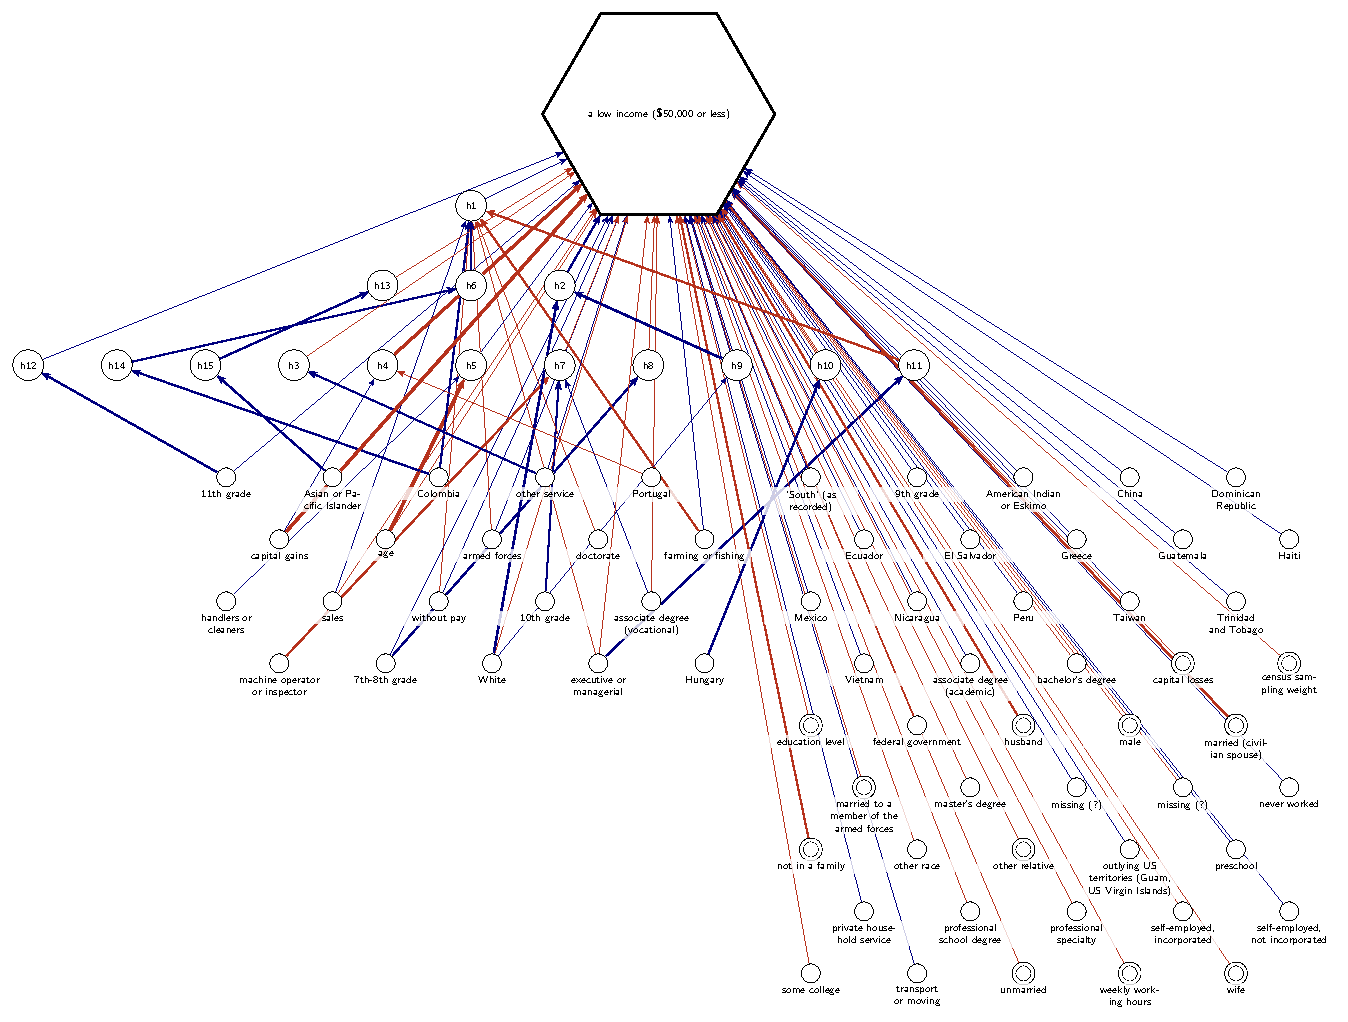
\includegraphics[width=\textheight,height=0.78\textwidth,keepaspectratio]{figures/exp2/networks/adult-s7-raw}
  \caption{Adult, seed 7 (adult-s7): the network as trained, before any explanation, in full. Inputs at the bottom (every input column its own node), hidden units by depth, the output at the top; 65 of 107 input columns are connected, with 15 hidden units and 95 enabled connections. Blue: positive weight (raises the score); red: negative weight (lowers it); thicker: larger weight. Orange outline and up arrow: raises the final prediction; teal and down arrow: lowers it; grey and double arrow: depends. Not used (no connection; 42 columns): local government, private, state government, high-school graduate, 12th grade (no diploma), 1st-4th grade, 5th-6th grade, divorced, married, spouse absent, never married, separated, widowed, administrative or clerical, protective service, technical support, craft or repair, own child, Black, missing (?), Cambodia, France, Germany, the Netherlands, Honduras, Hong Kong, India, Canada, Iran, Ireland, Italy, Jamaica, Japan, Laos, the Philippines, Poland, Puerto Rico, Scotland, Thailand, the United States, Yugoslavia, Cuba and England.}
  \label{fig:exp2-net-adult-s7-raw}
\end{sidewaysfigure}
